\section{Project Plan}

The project plan provides a rough outline of all sprints, main activities and their respective time-frames. The project plan is represented as a Gantt-chart. The project is divided into nine sprints of about two weeks, and each sprint has it´s unique goal. The last sprints are not planned in full detail to give a buffer for unforeseen time and feature creep.

\subsection{Presentations}
During the project there are three presentations. Presentation one is in the start phase of the project, presentation two in the middle of the project and presentation three at the end of the project. A short description of what the different presentations will include is given below. \\\\
\begin{figure}[h]
\begin{minipage}[t]{0.5\textwidth}
\textbf{Presentation 1:}
\begin{itemize}
  \item Presentation of team members
  \item Introduction to the project
  \item The method of execution
  \item Describe the process and project model 
  \item Project plan
  \item Requirements specification
  \item Test specification 
\end{itemize}
\end{minipage}
\hfill
\begin{minipage}[t]{0.5\textwidth}
\textbf{Presentation 2:}
\begin{itemize}
  \item The chosen solution
  \item Present the projects progress
  \item Explain testing
  \item Present the plan forward
\end{itemize}
\end{minipage}
\hfill
\end{figure}\\
\\
\textbf{Presentation 3:}
This presentation is divided into two main parts of 20 minutes. The first part is a sales pitch for the product. The second part is a technical presentation of the product. \\
The first part will describe:
\begin{itemize}
  \item Why the product/solution is the best 
  \item Mention the positive sides of the product
  \item Compare the product to other products 
\end{itemize}
The second part will describe: 
\begin{itemize}
  \item What the team has learned during the project 
  \item The teams time usage 
  \item The technical solution
  \item A conclusion to the project 
\end{itemize} 

\subsection{Milestones}
In order to complete this project, a list of the milestones have been made. The milestones represent the important events throughout the projects life time and when they are expected to be accomplished. 
\\\\
Some of the intention behind the milestones is to gain insight and understanding of the tasks to be solved. The milestones give an overview of the work to be done, and a base for committing resources. The goal is to have a good overview of the progress in the project. The Gantt-chart however, gives a detailed overview of all activities in the entire project from start to finish. Milestones are a way to summarize tasks into larger pieces and keep track of the project development. They give a clear deadline for when these tasks should be done. Deadlines are set to have a greater efficiency and progress. It provides information to the stakeholders of what they can expect of progress and when the various stages will be completed.\\
\begin{table}[h]

\centering\section*{\textbf{Milestones}}
\caption{Milestones}
\begin{tabular}{llc}
\rowcolor{cadetgrey}
\centering \textbf{Milestone:}    &\textbf{Description:} 	 &\textbf{Expected done:} \\ % &\textbf{Main responsibility:}  \\

\rowcolor{gainsboro}
\textbf{Requirements Identification} & Identify requirements and needs & $13.01.17$ \\
\textbf{Project Plan} & Create a project plan, divide activities, & $24.01.17$ \\
                                     & plan organization & \\
\rowcolor{gainsboro}
\textbf{First Prototype} & Create a simple fixed pitch & $14.02.17$ \\\rowcolor{gainsboro}
                         & quadcopter to test & \\\rowcolor{gainsboro}
                         & flight controller & \\
\textbf{Preliminary Design} & Create a preliminary design & $21.02.17$ \\
                            & for fixed and variable pitch & \\\rowcolor{gainsboro}
\textbf{Basic PID controller} & Develop basic PID controller & $21.02.17$ \\\rowcolor{gainsboro}
                                 & For a fixed and & \\\rowcolor{gainsboro}
                                 & variable pitch quadcopter & \\
\textbf{Basic Flight Controller} & Create a basic flight controller & $28.02.17$ \\
                                 & so the quadcopter can elevate, & \\
                                 & land and go left and right & \\\rowcolor{gainsboro}
\textbf{Fixed Pitch Quadcopter} & Create the fixed pitch quadcopter & $13.03.17$ \\\rowcolor{gainsboro}
                                & (no more changes have been planned) & \\
\textbf{Flight Controller FPQ}  & Finish a flight controller for fixed & $28.03.17$ \\
                                & pitch with possibility for autonomous & \\
                                & and agile flying & \\\rowcolor{gainsboro}
\textbf{Variable Pitch Quadcopter}  & Create the variable pitch quadcopter & $28.03.17$ \\\rowcolor{gainsboro}
                                    & (no more changes have been planned) & \\
\textbf{Flight Controller VPQ}  & Finish a flight controller for variable & $28.04.17$ \\
                            & pitch with possibility for autonomous & \\
                            & and agile flying & \\\rowcolor{gainsboro}
\textbf{Compare fixed and variable pitch}  & Test and compare the quad- & $14.05.17$ \\\rowcolor{gainsboro}
                                           & copters to answer the main & \\\rowcolor{gainsboro}
                                           & requirements & 
\end{tabular}                                                               
\end{table}

\begin{table}[h]

\centering\section*{\textbf{Milestones - Done, Moved, Not Completed}}
\caption{Milestones - so far}
\begin{tabular}{llc}
\rowcolor{cadetgrey}
\centering \textbf{Milestone:}    &\textbf{Description:} 	 &\textbf{Expected done:} \\ % &\textbf{Main responsibility:}  \\

\rowcolor{green}
\textbf{Requirements Identification} & Identify requirements and needs & $13.01.17$ 
\\\rowcolor{green}
\textbf{Project Plan} & Create a project plan, divide activities, & $24.01.17$ \\\rowcolor{green}

                                     & plan organization & \\
\rowcolor{green}
\textbf{First Prototype} & Create a simple fixed pitch & $14.02.17$ \\\rowcolor{green}
                         & quadcopter to test & \\\rowcolor{green}
                         & flight controller & 
                         \\\rowcolor{green}
\textbf{Preliminary Design} & Create a preliminary design & $21.02.17$ 
\\\rowcolor{green}
                            & for fixed and variable pitch & \\\rowcolor{green}
\textbf{Basic PID controller} & Develop basic PID controller & $21.02.17$ \\\rowcolor{green}
                                 & For a fixed and & \\\rowcolor{green}
                                 & variable pitch quadcopter & \\\rowcolor{green}
\textbf{Basic Flight Controller} & Create a basic flight controller & $28.02.17$ \\\rowcolor{green}
                                 & so the quadcopter can elevate, & \\\rowcolor{green}
                                 & land and go left and right & \\\rowcolor{green}
\textbf{Fixed Pitch Quadcopter} & Create the fixed pitch quadcopter & $13.03.17$ \\\rowcolor{green}
                                & (no more changes have been planned) & \\\rowcolor{yellow}
\textbf{Flight Controller FPQ}  & Finish a flight controller for fixed & $28.03.17$ \\\rowcolor{yellow}
                                & pitch with possibility for autonomous & \\\rowcolor{yellow}
                                & and agile flying & \\\rowcolor{yellow}
\textbf{Variable Pitch Quadcopter}  & Create the variable pitch quadcopter & $28.03.17$ \\\rowcolor{yellow}
                                    & (no more changes have been planned) & \\
\textbf{Flight Controller VPQ}  & Finish a flight controller for variable & $28.04.17$ \\
                            & pitch with possibility for autonomous & \\
                            & and agile flying & \\\rowcolor{gainsboro}
\textbf{Compare fixed and variable pitch}  & Test and compare the quad- & $14.05.17$ \\\rowcolor{gainsboro}
                                           & copters to answer the main & \\\rowcolor{gainsboro}
                                           & requirements & 
\end{tabular}                                                               
\end{table}
\vspace{3cm}
\noindent
The table above shows the progress so far in the project. Green indicates completed milestones, and yellow indicates incomplete milestones. In sprint 4 (10.03) some milestones were not reached, so the project plan and milestones had to be reevaluated. The team then contacted the customer to brief them on the project status. In this meeting it was concluded that FFI was mainly interested in stable landing. This information was taken into consideration when the second project plan and milestones were created.
\\\\
The table on the next page illustrates the new milestones for the project. It is mostly the same, some dates have been changed, and one task is added. This task is radio control for variable pitch quadcopter.

\begin{table}[H]

\centering\section*{\textbf{Milestones - Reworked}}
\caption{Milestones - reworked}
\begin{tabular}{llc}
\rowcolor{cadetgrey}
\centering \textbf{Milestone:}    &\textbf{Description:} 	 &\textbf{Expected done:} \\ % &\textbf{Main responsibility:}  \\

\rowcolor{gainsboro}
\textbf{Requirements Identification} & Identify requirements and needs & $13.01.17$ \\
\textbf{Project Plan} & Create a project plan, divide activities, & $24.01.17$ \\
                                     & plan organization & \\
\rowcolor{gainsboro}
\textbf{First Prototype} & Create a simple fixed pitch & $14.02.17$ \\\rowcolor{gainsboro}
                         & quadcopter to test & \\\rowcolor{gainsboro}
                         & flight controller & \\
\textbf{Preliminary Design} & Create a preliminary design & $21.02.17$ \\
                            & for fixed and variable pitch & \\\rowcolor{gainsboro}
\textbf{Basic PID controller} & Develop basic PID controller & $21.02.17$ \\\rowcolor{gainsboro}
                                 & For a fixed and & \\\rowcolor{gainsboro}
                                 & variable pitch quadcopter & \\
\textbf{Basic Flight Controller} & Create a basic flight controller & $28.02.17$ \\
                                 & so the quadcopter can elevate, & \\
                                 & land and go left and right & \\\rowcolor{gainsboro}
\textbf{Fixed Pitch Quadcopter} & Create the fixed pitch quadcopter & $13.03.17$ \\\rowcolor{gainsboro}
                                & (no more changes have been planned) & \\
\textbf{Variable Pitch Quadcopter}  & Create the variable pitch quadcopter & $11.04.17$ \\
                                    & (no more changes have been planned) & \\\rowcolor{gainsboro}
\textbf{Radio Control VPQ}  & Modify a fixed pitch flight controller & $18.04.17$ \\\rowcolor{gainsboro}
                                & to work with radio control & \\
\textbf{Flight Controller VPQ}  & Finish a flight controller for variable & $09.05.17$ \\
                            & pitch with possibility for autonomous & \\
                            & and agile flying & \\\rowcolor{gainsboro}
\textbf{Compare fixed and variable pitch}  & Test and compare the quad- & $16.05.17$ \\\rowcolor{gainsboro}
                                           & copters to answer the main & \\\rowcolor{gainsboro}
                                           & requirements & 
\end{tabular}                                                               
\end{table}

\subsection{Activity List}

The purpose of identifying the project activities is to get a sufficient estimate on what resources and time the project will require to be completed. Activities are usually given an expected duration and resource use, in terms of manpower, knowledge and budget. 
The list tends to be extensive containing all scheduled activities in the project. Scrum on the other hand doesn't plan when every activity should be done. The first phase in a Scrum project is to make a product road map, which can be done in as little as a day. Scrum gets an advantage by cutting the planning process, but in return struggles with getting the project done within a given time-frame. Since we can't move the end date of the project, Scrum needs to be modified a little in order to meet our project needs. 
\\\\
In this project a mix of the traditional long-term planning and Scrum is used. The process of identifying activities uses decomposition to break down the structure of larger tasks (such as milestones and backlog items). Activities are identified by asking "What has to be done" often in form of functionality. Then the functionality are translated into milestones and larger activities.
\\\\
A plan for all the project sprints are made, as well as using the advantage of Scrum by planning each sprint in-depth. Combining the sprints with an overall project plan helps by reaching the end date and still keep Scrum's feedback and agility. You can find a list of the initial activities that have been identified at this point in the project beneath. 
\\\\
To get an overview of the project plan a Gantt-Chart is used. By using a Gantt-Chart the team get the advantage of having an overview of the project and its associated tasks. With a Gantt-chart you could see all this information at a glance. Usually, the most critical activities and milestones are represented in the Gantt-Chart. The chart is frequently used in project management, and are closely followed up by the project leader in order to meet the deadline.
\\\\

\begin{center}
\centering\section*{\textbf{Activity Layout}}
%\caption{Activity Layout 1}
\begin{tabular}{cllll}
\rowcolor{cadetgrey}
\textbf{ID:}    &\textbf{Activity:} 	 &\textbf{Estimated time:}    &\textbf{Start:}  \\ % &\textbf{Main responsibility:}  \\
    
\textbf{1} & \textbf{Start-Up Phase} & \textbf{260h} & $03.01.17$ 
\\\rowcolor{gainsboro}
1.1       & Documentations     &     &  \\
1.2       & Research     &     &  \\\rowcolor{gainsboro}
1.3       & Project Model     &     & \\
1.4       & Project Plan     &     & 
\\\rowcolor{gainsboro}
1.5       & Requirements     &     & \\
1.6       & Test Specification     &     & 
\\\rowcolor{gainsboro}
1.7       & Document Templates     &    & \\
1.8       & Internal Meetings      &    & 
\\\rowcolor{gainsboro}
1.9       & External Meetings      &    & \\
\textbf{2} & \textbf{Presentation 1}     & \textbf{100h}    & $03.01.17$ 
\\\rowcolor{gainsboro}
2.1     & Preliminary Documentation Refinement  &    & \\
2.2     & Presentation Refinement  &    &
\\\rowcolor{gainsboro}
2.3     & Presentation Practice  &    & \\
\textbf{3} & \textbf{Sprint 1}     & \textbf{360h}     & $17.01.17$ 
\\\rowcolor{gainsboro}
3.1     & First Presentation &  & \\
3.2     & Preliminary Flight Simulation &  & 
\\\rowcolor{gainsboro}
3.3     & Communication With Qualisys &  & \\
3.4     & Mechanical Design Study &  & 
\\\rowcolor{gainsboro}
3.5       & Internal Meetings      &    & \\
3.6       & External Meetings      &    & 
\\\rowcolor{gainsboro}
\textbf{4} & \textbf{Sprint 2}     & \textbf{360h}     & $31.01.17$ \\
4.1     & Electrical Analysis &  &  \\\rowcolor{gainsboro}
4.2     & Electrical Layout &  & \\
4.3     & Electrical Construction & & \\ \rowcolor{gainsboro}
4.4     & Flight Controller & & \\
4.5     & Create Web Page & &  
\\\rowcolor{gainsboro}
4.6     & Mechanical Design & & \\
4.7     & Preliminary Construction & & 
\\\rowcolor{gainsboro}
4.8       & Internal Meetings      &    & \\
4.9       & External Meetings      &    & 
\end{tabular}                                                                   
\end{center}
\newpage

\begin{center}
\section*{\textbf{Activity Layout}}
%caption{Activity Layout 2}
\begin{tabular}{cllll}
\rowcolor{cadetgrey}
\textbf{ID:}    &\textbf{Activity:} 	 &\textbf{Estimated time:}    &\textbf{Start:}  \\ % &\textbf{Main responsibility:}  \\
\rowcolor{gainsboro}
\textbf{5} & \textbf{Sprint 3}     & \textbf{360h}     & $14.02.17$ \\
5.1     & Plan Test Procedures &  &  \\\rowcolor{gainsboro}
5.2     & Mechanical Design &  &  \\
5.3     & Preliminary Variable Pitch Design & & 
\\\rowcolor{gainsboro}
5.4     & Flight Testing and Controll &  & \\
5.5       & Internal Meetings      &    & 
\\\rowcolor{gainsboro}
5.6       & External Meetings      &    & \\
\textbf{6} & \textbf{Sprint 4}     & \textbf{360h}     & $28.02.17$ \\
\rowcolor{gainsboro}
6.1     & Mechanical Design Review & & \\
6.2     & Tweak Flight Controller & & 
\\\rowcolor{gainsboro}
6.3       & Internal Meetings      &    & \\
6.4       & External Meetings      &    & 
\\\rowcolor{gainsboro}
\textbf{7} & \textbf{Sprint 5}     & \textbf{360h}     & $14.03.17$ \\
7.1     & Advanced Controll Functionality &  & \\\rowcolor{gainsboro}
7.2       & Internal Meetings      &    & \\
7.3       & External Meetings      &    & 
\\\rowcolor{gainsboro}
\textbf{8} & \textbf{Presentation 2}     & \textbf{100h}     & $28.03.17$ \\
8.1     & Presentation 2 planning &  &  \\\rowcolor{gainsboro}
\textbf{9} & \textbf{Sprint 6}     & \textbf{360h}     & $28.03.17$ \\
9.1     & Finalize Test Procedures &  & 
\\\rowcolor{gainsboro}
9.2     & Tweak Controller System &  & \\
9.3       & Internal Meetings      &    & 
\\\rowcolor{gainsboro}
9.4       & External Meetings      &    & \\
\textbf{10} & \textbf{Sprint 7}     & \textbf{460h}     & $11.04.17$ \\
\rowcolor{gainsboro}
10.1     & Final Flight Controller Adjustment &  & \\
10.2     & Testing and Comparison & & 
\\\rowcolor{gainsboro}
10.3       & Internal Meetings      &    & \\
10.4       & External Meetings      &    & 
\\\rowcolor{gainsboro}
\rowcolor{gainsboro}
\textbf{11} & \textbf{Sprint 8}     & \textbf{460h}    & $25.04.17$ \\
11.1     & Testing and Comparison              &  &  \\\rowcolor{gainsboro}
11.2     & Documentation &  &  \\
11.3     & Testing & &  \\\rowcolor{gainsboro}
11.4       & Internal Meetings      &    & \\
11.5       & External Meetings      &    & 
\\\rowcolor{gainsboro}
\rowcolor{gainsboro}
\textbf{12} & \textbf{Sprint 9}     & \textbf{460h}     & $09.05.17$ \\
12.1     & Testing and Comparison &  &  \\\rowcolor{gainsboro}
12.2     & Documentation Review &  & \\
12.3       & Internal Meetings      &    & 
\\\rowcolor{gainsboro}
12.4       & External Meetings      &    & \\
\textbf{13} & \textbf{Presentation 3}     & \textbf{100h}     & $09.05.17$ \\
\rowcolor{gainsboro}
13.1     & Documentation Review &  & \\
13.2     & Practice & & \\
\rowcolor{gainsboro}
         & \textbf{Total amount of hours estimated:} & \textbf{4200h} & 
         \\\\\\\\\
\end{tabular}                                                               
\end{center}

\begin{comment}
\subsection{Gantt-chart}

Imagine being a juggler, juggling a lot of balls. The more balls you have in the air, the harder it gets keeping track of everything. In addition the more balls we have in the air, the more mess it can potentially be if something starts to slip out of hand. Being a juggler and being a system engineer are similar when it comes to this. The engineer needs to keep track of all the activities in the project, if he does not accomplish this, then the project will surely fail. Failure to deliver a task or a sequence of tasks within a given deadline, can have direct or indirect effect on the rest of the project. This may affect the end date of the project as well as the cost.\\
\\
This is why it is advantageous to have an overview of the project and its associated tasks. With a Gantt-chart you could see all this information at a glance. Usually, the most critical activities and milestones are represented in the Gantt-chart. Gantt-charts are an important tool when it comes to visualisation of activities. It is frequently used in project management, and are closely followed up by the project leader in order to meet the deadline. The chart has a list of the tasks on the left and information about the start, duration, relationship to other tasks and end date as a timeline to the right. The Gantt-chart is provided as a separate document. \\
\end{comment}

\begin{comment}
Things that should be in a project plan/ description:

Scope management
Schedule management
Financial management
Quality management
Resource management
Stakeholder management – New from PMBOK 5[citation needed]
Communications management
Project change management
Risk management
\end{comment}

\subsection{Budget}
The project has a budget of 10.000 NOK. The budget will mainly be used to purchase quadcopter parts. A small amount of the budget is used on project management tools, such as Jira and sharelatex. If the team encounter unforeseen expenses, FFI has approved that the budget may be stretched to 15.000 NOK.
\\\\
In Fig. \ref{fig:budget} you can see our budget so far. In the middle of Sprint 5 the original budget of 10.000 NOK was exceeded. Parts and supplies are expensive and made it impossible to stay within the budget of 10.000 NOK. The budget was therefore extended to 15.000 NOK. 

\begin{figure}[H]
    \centering
    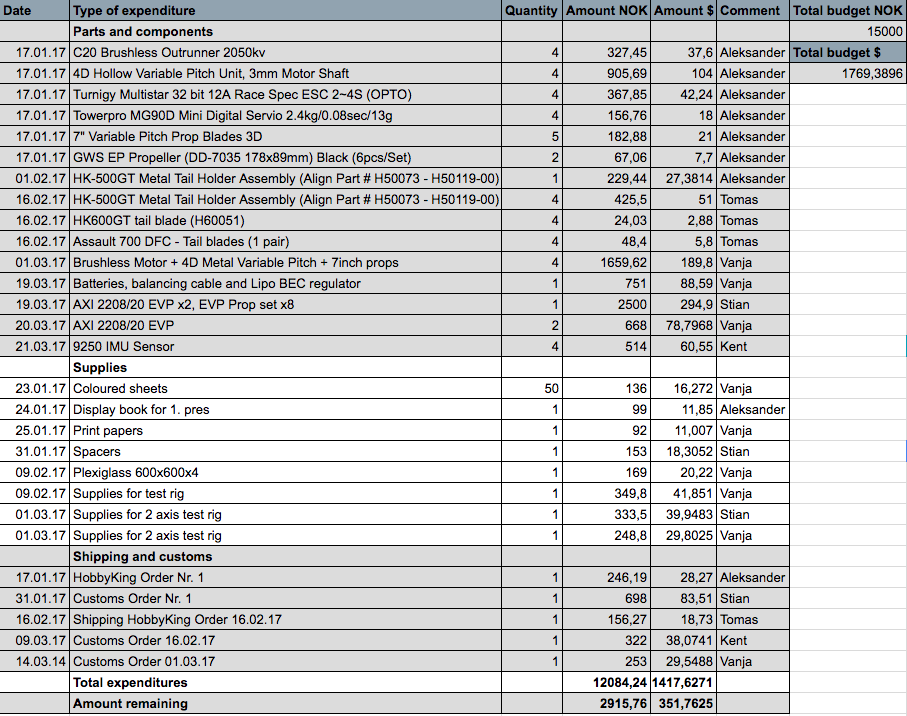
\includegraphics[width = 1.0\textwidth]{VAPIQ-PICTURES/budget1.png}
    \caption{VAPIQ Budget}
    \label{fig:budget}
\end{figure}
\\

\newpage
\subsection{Risk Management}
During the start-up phase, and trough out the project, it is important to do a thorough risk analysis, so a plan to scenarios that could endanger and have a negative impact on our project can be made. If a risk is not taken care of, it can interrupt the progress of the project, and eventually the outcome of the project.
\\\\ 
The risk analysis identifies all possible scenarios that can cause problems for the project development, and determines the probability and severity of these scenarios. By identifying these scenarios it can minimize, or eliminate the risks. It is important to always reevaluate the risks at every sprint, in order to keep track of current risks or identify new ones.
\\\\
\begin{figure}[H]
    \centering
    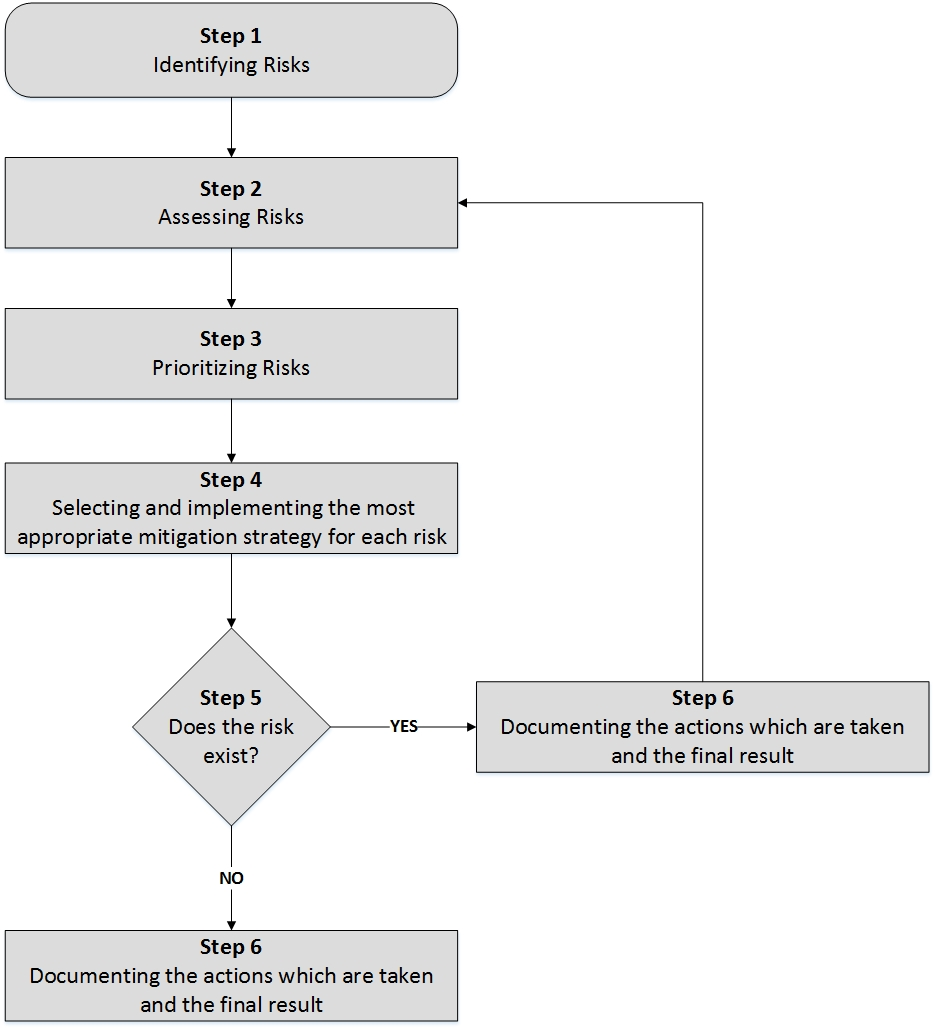
\includegraphics[width = 0.7\textwidth]{VAPIQ-PICTURES/riskprocess.jpg}
    \caption{Risk Identification Process}
    \label{fig:riskid}
\end{figure}
\clearpage
\noindent
Fig. \ref{fig:riskid} shows the risk identification process the team are using. Fig. \ref{fig:riskid} are taken from \cite{Alberto}.

\begin{comment}
Examples of risk scenarios are budget overrun, injuries, long term sick-leave etc. The scenarios are categorized with the probability of occurrence and the severity of this scenario. The scenarios are further analysed in a risk matrix which helps us to see which risks are most critical for the project.
\end{comment}
\\\\\noindent
Three categories to analyze the risk scenarios were used:
\begin{itemize}
\item{Likelihood of occurrence}
\item{Severity of the scenario}
\item{Detectability (how easy it is to detect the risk scenario)}
\end{itemize}
All risk scenarios are rated according to these three categories with low, medium and high ranking. A likelihood of high, means that the scenario is most likely to happen. High severity means that the consequences are severe if it happens. And high detectability means that it is hard to detect the scenario, so they are unlikely to be discovered by the team.
\\\\
A risk assessment matrix was developed based on the likelihood of occurrence, severity of the scenario and detectability. This matrix can be seen in Fig. \ref{AssRisk}. This matrix is a very helpful tool to visualize the risk, and how critical it is. A risk is defined as the product between the probability of occurrence times the severity. 

$$Risk = Likelihood\cdot Severity$$ 
\\
The Risk assessment matrix is used to determine which Strategy of Action to be implemented on each risk. 

\begin{figure}[H]
    \centering
    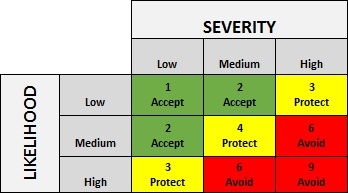
\includegraphics[width = 0.4\textwidth]{VAPIQ-PICTURES/RiskAss.jpg}
    \caption{Risk assesment matrix}
    \label{AssRisk}
\end{figure}
\\\\ \noindent
Three Strategies of Actions (SOA) were developed to handle any risk. Strategies of Actions are any action that can reduce or eliminate the chance of a risk to appear. Strategies of Actions can also be actions that can decrease the severity of the consequences. The Strategies of Action are:
\begin{itemize}
\item{Accept: Risks with low ranking. No action is needed on these risks. No imminent danger.}
\item{Protect: Risks with medium ranking. These risks requires actions to reduce the probability of occurrence.}
\item{Avoid: Risks with high ranking. These risks need to be eliminated or reduced. If the risk occurs, a plan to handle the risk needs to be developed.}
\end{itemize}
\\\\
For Strategies of Acting including Protect and Avoid, there need to be developed a plan on how to handle the risk. These plans are called Mitigation Strategy and can be shown in Appendix B3.
\\\\
Appendix B3 also shows all the different risk scenarios, along with the strategies, likelihood, severity, detectability and origin. Every scenario has a unique ID for easy traceability.

\\\\\noindent
\begin{comment}
After analysing all scenarios in the risk assessment matrix, we know that, for instant, sudden new requirements from the customer FFI, can put the project at risk. This is because of limited time and a deadline that is fixed. If this happens we need to adapt and accept it, change the backlog and re-prioritize activities. And since we are using the highly iterative scrum model, it is relatively easy to handle changes. The risk which got the highest rating was wrong estimation of story-points. Estimating wrong will put the whole project in danger in the way that we don't have a product at the end. Most of the highest risks, are connected to requirements. Thus we need to always reevaluate user stories at every sprint review meeting in order to ensure completeness. Budget overrun also is a huge risk. Therefore it is important to do thorough studies before we decide to order parts.
\\\\
To ensure low risk it is important to have a risk meeting at the beginning of each sprint. Here we reevaluate the risk scenarios, and analyzes which risks that are most likely to happen during the sprint. During these meetings we must develop plans on how to handle the risks that are most likely to happen.
\end{comment}

